% How the data of the benchmark is made: clean test sets, noisy test sets, fine-tuning data.
% The numbers and checksums come from the .meta.json files next to each data file (2026-11-24).
%   cd docs/reports/data && latexmk -pdf data_generation.tex
\documentclass[10pt,a4paper]{article}
\usepackage[T1]{fontenc}
\usepackage{lmodern}
\usepackage[margin=2cm]{geometry}
\usepackage{microtype}
\usepackage{amsmath}
\usepackage{booktabs}
\usepackage{tabularx}
\usepackage{xcolor}
\usepackage{enumitem}
\usepackage{tikz}
\usetikzlibrary{positioning,arrows.meta}
\usepackage{caption}
\usepackage[hidelinks]{hyperref}
\captionsetup{font=small,labelfont=bf,skip=4pt}
\setlist{itemsep=1pt,topsep=3pt}
\setlength{\parindent}{0pt}
\setlength{\parskip}{4pt}
\newcommand{\file}[1]{\texttt{#1}}
\newcommand{\rx}[1]{\mbox{\small\texttt{#1}}}
\newcolumntype{L}{>{\raggedright\arraybackslash}X}

\begin{document}

\begin{center}
{\Large\bfseries PIIGuard: how the data is made}\\[3pt]
{\small Clean test sets, noisy test sets and fine-tuning data \textperiodcentered{} CSED490E, PIIGuard team
\textperiodcentered{} November 24, 2026}
\end{center}

This document gives the procedure behind every data file of the benchmark, step by step, so that
anyone can make the same files again and check that they are the same. The data files themselves
are not in git (dataset licenses; see the README); they are rebuilt with the scripts below. The
training procedure is in \file{docs/reports/train/training\_procedure.pdf}; the results are in
the Q2/Q3 report, \file{docs/reports/q2\_q3/}.

\section{Overview}

\begin{center}
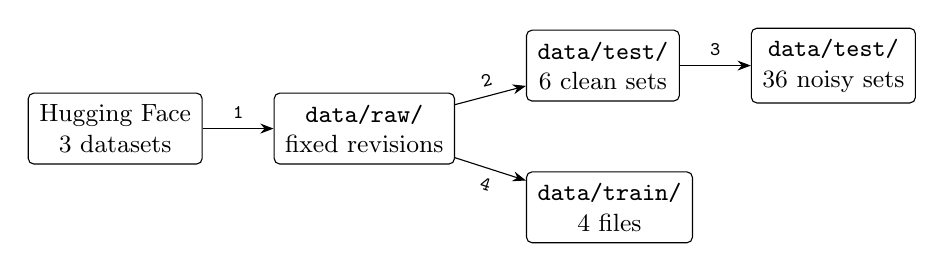
\begin{tikzpicture}[node distance=5mm and 9mm, box/.style={draw, rounded corners=2pt, align=center, font=\small,
  inner sep=4pt, minimum height=9mm}, lab/.style={font=\scriptsize\ttfamily, midway, above}, >=Stealth]
\node[box] (hf) {Hugging Face\\ 3 datasets};
\node[box, right=of hf] (raw) {\file{data/raw/}\\ fixed revisions};
\node[box, right=of raw, yshift=8mm] (clean) {\file{data/test/}\\ 6 clean sets};
\node[box, right=of clean] (noisy) {\file{data/test/}\\ 36 noisy sets};
\node[box, right=of raw, yshift=-10mm] (train) {\file{data/train/}\\ 4 files};
\draw[->] (hf) -- node[lab]{1} (raw);
\draw[->] (raw) -- node[lab, sloped]{2} (clean);
\draw[->] (clean) -- node[lab]{3} (noisy);
\draw[->] (raw) -- node[lab, sloped, below]{4} (train);
\end{tikzpicture}
\end{center}

\begin{tabularx}{\linewidth}{@{}clLr@{}}
\toprule
Step & Script & Output & Time \\
\midrule
1 & \file{experiments/download\_data.py} & \file{data/raw/<dataset>/}: the files of each dataset at a fixed revision & minutes \\
2 & \file{experiments/prepare\_data.py} & \file{data/test/<dataset>\_clean[\_dates]}: the clean test sets (question 1) & seconds \\
3 & \file{experiments/make\_noisy.py} & \file{data/test/<dataset>\_noisy\_<kind>[\_dates]}: the noisy test sets (question 2) & about 10 s \\
4 & \file{experiments/prepare\_train.py} & \file{data/train/ai4privacy\_<part>\_<version>.jsonl}: the fine-tuning data (question 3) & about 15 s \\
\bottomrule
\end{tabularx}

{\small
\begin{verbatim}
uv run python experiments/download_data.py
uv run python experiments/prepare_data.py
uv run python experiments/make_noisy.py
uv run python experiments/prepare_train.py
\end{verbatim}
}

Every data file is JSON Lines, one example per line, with the fields \file{id}, \file{text},
\file{spans} (each with \file{start}, \file{end} and \file{label}, character offsets into
\file{text}) and \file{meta}. Next to each file, a \file{.meta.json} records where it comes from, its seeds, the
number of gold spans per label and its SHA-256 checksum (Section~\ref{sec:checksums}).

\section{Sources (step 1)}

\begin{tabularx}{\linewidth}{@{}lllL@{}}
\toprule
Dataset & Repository & Revision & Part used \\
\midrule
ai4privacy & \file{ai4privacy/open-pii-masking-500k-ai4privacy} & \file{506996d625} & validation split (test sets; there is no test split), train split (fine-tuning); English records only \\
Nemotron-PII & \file{nvidia/Nemotron-PII} & \file{b70ffaf5ff} & test split (100,000 English documents, locales \file{us} and \file{intl}) \\
Gretel & \file{gretelai/synthetic\_pii\_finance\_multilingual} & \file{7b844d1673} & test split, English records (2,962 of 5,594) \\
\bottomrule
\end{tabularx}

The revisions are pinned in \file{benchmark/data.py}, so a later change of a dataset on Hugging
Face does not change our files. Nemotron-PII and Gretel are used for testing only: their train
splits are not downloaded.

\section{Labels and span clean-up}

Each dataset's labels are mapped to our six labels (\file{benchmark/data.py}); every other
dataset label is dropped. The \file{\_dates} versions (comparison C) put every date under
\file{DATE} instead of keeping \file{DATE\_OF\_BIRTH}.

\begin{tabularx}{\linewidth}{@{}lLLL@{}}
\toprule
Our label & ai4privacy & Nemotron-PII & Gretel \\
\midrule
NAME & GIVENNAME, SURNAME & first\_name, last\_name & name, first\_name, last\_name \\
EMAIL & EMAIL & email & email \\
PHONE & TELEPHONENUM & phone\_number & phone\_number \\
ADDRESS & BUILDINGNUM, STREET & street\_address & street\_address \\
DATE\_OF\_BIRTH & (none) & date\_of\_birth & date\_of\_birth \\
CARD\_NUMBER & CREDITCARDNUMBER & credit\_debit\_card & credit\_card\_number \\
\midrule
DATE (\file{\_dates} only) & DATE & date, date\_of\_birth, date\_time & date, date\_of\_birth, date\_time \\
\bottomrule
\end{tabularx}

ai4privacy marks only the building number and the street as an address (city, zip code and
flat number are other labels, dropped here); Nemotron-PII and Gretel mark more of the address.
This difference matters for question 3 (see the Q2/Q3 report, Section 6.1).

The same clean-up (\file{benchmark/spans.py}) is applied to the gold spans of every dataset and to
every detector's output:
\begin{enumerate}
\item drop spans outside the text, and move span edges inward past whitespace and past a pair of
  brackets or quotes around the whole span (\file{[x@y.com]} $\to$ \file{x@y.com});
\item remove a leading title from NAME spans (\file{Dr. Kim} $\to$ \file{Kim});
\item drop overlapping spans, keeping the one that starts first;
\item join spans with the same label that only spaces separate (\file{Minji} + \file{Park} $\to$ \file{Minji Park}).
\end{enumerate}

\section{Clean test sets (step 2)}

\file{experiments/prepare\_data.py} reads all English records of the split, maps the labels,
cleans the spans, and draws a random sample with seed 0 (\file{random.Random(0).sample} over the
record indices, kept in their original order). Records without any of our labels are kept: they
test whether a detector masks text that is not PII. The \file{\_dates} version holds the same
records in the same order, with the comparison-C labels.

{\small\setlength{\tabcolsep}{4.5pt}
\begin{tabular}{@{}lrrrrrrrrr@{}}
\toprule
Dataset & English & Drawn & NAME & EMAIL & PHONE & ADDRESS & DOB & CARD & DATE (C) \\
\midrule
ai4privacy & 30,160 & 10,000 & 8,748 & 1,185 & 1,567 & 1,533 & -- & 185 & 1,387 \\
Nemotron-PII & 100,000 & 2,000 & 2,053 & 1,091 & 464 & 324 & 363 & 257 & 2,126 \\
Gretel & 2,962 & 2,962 & 4,475 & 837 & 531 & 2,322 & 143 & 76 & 5,768 \\
\bottomrule
\end{tabular}}

English: English records of the split used. Gold spans per label; DATE (C) is the number of dates
in the \file{\_dates} version.

The sizes were fixed after timing the detectors, so that questions 1 to 3 fit on laptop CPUs.

\section{Noisy test sets (step 3)}

\file{experiments/make\_noisy.py} makes, for each clean test set and each kind of noise, a copy
with the same examples and ids, using \file{benchmark/noise.py}. The kinds follow Section 4.2 of
the proposal.

\subsection{Where each kind can edit, and how}

\begin{tabularx}{\linewidth}{@{}l>{\raggedright\arraybackslash}p{4.6cm}L@{}}
\toprule
Kind & Candidate places (regular expression) & Edit \\
\midrule
\file{typo} & words of 3+ letters, \rx{[A-Za-z]\{3,\}} & one of four, at random: a letter added (the same letter again, or a neighbouring key), a letter dropped, two different neighbouring letters swapped, a letter replaced by a neighbouring key (QWERTY rows, and the keys above and below) \\
\file{space} & one space between two words, \rx{(?<=\textbackslash S)\textvisiblespace(?=\textbackslash S)}; or a word of 4+ letters, \rx{[A-Za-z]\{4,\}} & the space dropped; or a space added inside the word, never at its first or last letter \\
\file{case} & words with a capital, \rx{[A-Za-z]*[A-Z][A-Za-z]*} & the word in lowercase \\
\file{punct} & \rx{[.,;:!?]} followed by a space or the end of the text & the mark dropped (so \file{x@y.com} and \file{1,234} are never touched) \\
\file{number} & digit groups with separators, \rx{\textbackslash d+(?:[\textvisiblespace\textbackslash -./]\textbackslash d+)+} & with probability 1/2 every separator dropped (\file{010-2345-6789} $\to$ \file{01023456789}); otherwise each separator replaced by a space, a hyphen or nothing, at random, until the result differs \\
\file{mixed} & all of the above & each edit of one of the five kinds \\
\bottomrule
\end{tabularx}

\subsection{Choosing the edits of one example}

\begin{enumerate}
\item \textbf{How many.} $n = \max(1, \mathrm{round}(0.10 \times \text{words}))$, words being the
  whitespace-separated tokens of the text. The rate 0.10 was fixed before any scoring.
\item \textbf{Random generator.} \file{random.Random("<seed>:<kind>:<example id>")} with seed 1, so
  each example's copy depends neither on the other examples nor on their order.
\item \textbf{Candidates.} For each kind allowed (one, or five for \file{mixed}), list its candidate
  places and shuffle them.
\item \textbf{Loop} until $n$ edits are kept or no candidate is left: pick at random a kind that
  still has candidates, take its next candidate, make the edit, and keep it unless
  \begin{itemize}
  \item it changes nothing;
  \item it crosses the edge of a gold span, in either the six-label or the \file{\_dates} spans
    (an edit is either inside a span or outside all spans);
  \item it overlaps an edit already kept;
  \item it would leave only spaces between two gold spans with the same label: the clean-up
    would then join them (\file{Roger Leblanc, Roger Leblanc} without its comma), and the noise
    would change the gold spans themselves.
  \end{itemize}
  A text with few places for a kind gets fewer edits; one with none is left as it is.
\item \textbf{Apply} the edits to the text, from the end to the start.
\end{enumerate}

\subsection{Moving the gold spans}

For a gold span $[s, e)$ and the kept edits, each with a length change
$\delta = |\text{new}| - |\text{old}|$:
\[
s' = s + \sum_{\text{edits ending at or before } s} \delta, \qquad
e' = e + \sum_{\text{edits ending at or before } e} \delta .
\]
A span keeps its label, even when an edit falls inside it (a misspelled email is still an email).
The moved spans are then cleaned with the four rules above. Both lists of spans (six labels and
\file{\_dates}) are moved with the same edits, so the two versions of a noisy copy have the same
text.

\subsection{Output and checks}

Each example's \file{meta.noise} holds the kind and the list of its edits
(\file{kind, start, end, old, new, inside}), \file{inside} telling whether the edit falls in a
gold span. There are 36 files: 3 datasets $\times$ 6 kinds $\times$ 2 label sets. Checks:
\begin{itemize}
\item every noisy set has exactly the same number of gold spans per label as its clean version
  (asserted for all 36 by \file{summarize\_data.py});
\item \file{tests/test\_noise.py} (2,411 tests): spans follow the text, no edit crosses an edge,
  edits per word, each kind edits only its places, the two span lists move together, the same
  seed gives the same copy, \file{mixed} uses every kind, two same-label values are never joined.
\end{itemize}

\begin{center}
\small
\begin{tabular}{@{}llrrrr@{}}
\toprule
Dataset & Copy & Examples changed & Edits & Edits per example & Inside a PII value \\
\midrule
ai4privacy & \texttt{typo} & 9{,}922 & 17{,}218 & 1.7 & 16.0\% \\
 & \texttt{space} & 9{,}923 & 17{,}219 & 1.7 & 10.8\% \\
 & \texttt{case} & 9{,}874 & 16{,}938 & 1.7 & 38.4\% \\
 & \texttt{punct} & 9{,}381 & 15{,}414 & 1.5 & 0.0\% \\
 & \texttt{number} & 2{,}487 & 2{,}609 & 0.3 & 58.5\% \\
 & \texttt{mixed} & 9{,}996 & 17{,}292 & 1.7 & 18.1\% \\
\midrule
Nemotron-PII & \texttt{typo} & 2{,}000 & 26{,}445 & 13.2 & 3.5\% \\
 & \texttt{space} & 2{,}000 & 26{,}445 & 13.2 & 2.4\% \\
 & \texttt{case} & 2{,}000 & 26{,}097 & 13.0 & 6.1\% \\
 & \texttt{punct} & 1{,}891 & 24{,}009 & 12.0 & 0.1\% \\
 & \texttt{number} & 1{,}711 & 4{,}674 & 2.3 & 23.3\% \\
 & \texttt{mixed} & 2{,}000 & 26{,}445 & 13.2 & 5.2\% \\
\midrule
Gretel & \texttt{typo} & 2{,}961 & 56{,}550 & 19.1 & 4.5\% \\
 & \texttt{space} & 2{,}956 & 56{,}574 & 19.1 & 3.6\% \\
 & \texttt{case} & 2{,}960 & 56{,}544 & 19.1 & 9.4\% \\
 & \texttt{punct} & 2{,}680 & 53{,}330 & 18.0 & 4.3\% \\
 & \texttt{number} & 1{,}992 & 8{,}297 & 2.8 & 8.6\% \\
 & \texttt{mixed} & 2{,}961 & 56{,}599 & 19.1 & 5.8\% \\
\bottomrule
\end{tabular}
\captionof{table}{Edits of each noisy test set (the \file{\_dates} versions have the same edits).
Source: \file{results/noise/test\_sets.md}.}
\end{center}

\section{Fine-tuning data (step 4)}

\file{experiments/prepare\_train.py} makes the data of question 3 from ai4privacy only, as Appendix
B of the proposal says.
\begin{enumerate}
\item Read the English records of the ai4privacy \textbf{train} split (120,533), with the
  comparison-C labels: every date is \file{DATE}, so that fine-tuning keeps BERT's date class.
  Our ai4privacy test set comes from the validation split, another split.
\item Hold out 5,000 records as a dev set: \file{random.Random(0).sample} over the record indices.
  The other 115,533 are the training set, in their original order.
\item Make one noisy copy of every record (training and dev): kind \file{mixed}, rate 0.10, the
  procedure of Section 5 with seed \textbf{2} instead of 1, so no noisy test copy is ever seen in
  training. The training copies have 201,528 edits (1.7 per record, 21\% inside a value).
\end{enumerate}

\begin{tabular}{@{}lrrrrrrr@{}}
\toprule
File & Records & NAME & EMAIL & PHONE & ADDRESS & DATE & CARD \\
\midrule
\file{ai4privacy\_train\_clean} & 115,533 & 101,783 & 13,282 & 17,984 & 17,487 & 16,391 & 2,148 \\
\file{ai4privacy\_train\_noisy} & 115,533 & \multicolumn{6}{c}{same spans as \file{train\_clean}} \\
\file{ai4privacy\_dev\_clean}, \file{\_noisy} & 5,000 each & 4,443 & 592 & 760 & 765 & 692 & 104 \\
\bottomrule
\end{tabular}

Version (a) of the fine-tuned BERT learns from \file{train\_clean}; version (b) from
\file{train\_clean} and \file{train\_noisy} together (231,066 records). The dev files are only
logged during training.

\textbf{Known overlap.} 89 of the 10,000 ai4privacy test sentences (0.9\%) also appear word for word
in the train split (the dataset repeats some sentences). Both fine-tuned versions saw them, so the
comparison between them is fair, but their in-domain scores are slightly optimistic.

\section{Checksums}\label{sec:checksums}

The first 16 hexadecimal digits of the SHA-256 of each file, as written in its \file{.meta.json}.
A file made again with the steps above must have the same checksum
(\file{sha256sum data/test/*.jsonl data/train/*.jsonl}).

\begin{center}
\small
\begin{tabular}{@{}lll@{}}
\toprule
Test set & six labels & \file{\_dates} \\
\midrule
\texttt{ai4privacy\_clean} & \texttt{4c24eefb4c9f2640} & \texttt{18cc95ddc5051a84} \\
\texttt{ai4privacy\_noisy\_typo} & \texttt{1edc4ba1f946f84c} & \texttt{f67115954af51e60} \\
\texttt{ai4privacy\_noisy\_space} & \texttt{910d478cb57d4b32} & \texttt{b6512077389d89e5} \\
\texttt{ai4privacy\_noisy\_case} & \texttt{2667127788b18a9a} & \texttt{907950b2e0f2dc1f} \\
\texttt{ai4privacy\_noisy\_punct} & \texttt{1342026a5c393494} & \texttt{d39dbcc4f93bce63} \\
\texttt{ai4privacy\_noisy\_number} & \texttt{97c92d84e920e9a5} & \texttt{5fd87961c8b69f24} \\
\texttt{ai4privacy\_noisy\_mixed} & \texttt{4ba4892d2cbf4c85} & \texttt{1125633d608b32ad} \\
\midrule
\texttt{nemotron\_clean} & \texttt{0e281bc30076928c} & \texttt{387d5dfa661af254} \\
\texttt{nemotron\_noisy\_typo} & \texttt{e30c0dee177238e5} & \texttt{536e590c89e067e2} \\
\texttt{nemotron\_noisy\_space} & \texttt{8fa19d6dccda0e9f} & \texttt{921b4812b8c0f88d} \\
\texttt{nemotron\_noisy\_case} & \texttt{6f37f02c54eca22e} & \texttt{08b9214df3b43625} \\
\texttt{nemotron\_noisy\_punct} & \texttt{4faa354fba68f266} & \texttt{ab15f41bfcb86b9e} \\
\texttt{nemotron\_noisy\_number} & \texttt{7e92cab95a272f58} & \texttt{76bea3b8d1c009b5} \\
\texttt{nemotron\_noisy\_mixed} & \texttt{59304999297df571} & \texttt{d26279640dff3f1d} \\
\midrule
\texttt{gretel\_clean} & \texttt{33689f6ea1a0098b} & \texttt{e25aa8cfe5e18630} \\
\texttt{gretel\_noisy\_typo} & \texttt{e7b96289c613189a} & \texttt{e3b0e80d31227db9} \\
\texttt{gretel\_noisy\_space} & \texttt{db47af3cfd7d6803} & \texttt{a93d9545c5917b67} \\
\texttt{gretel\_noisy\_case} & \texttt{dab022c140db446f} & \texttt{bd144745e9aa8d02} \\
\texttt{gretel\_noisy\_punct} & \texttt{6abb7389b6d0d348} & \texttt{9c20344eae730315} \\
\texttt{gretel\_noisy\_number} & \texttt{56e236d0a61b42f5} & \texttt{e3cb1d3bfa45c654} \\
\texttt{gretel\_noisy\_mixed} & \texttt{dbba2df31d1d8165} & \texttt{459eae6b1d910132} \\
\bottomrule
\end{tabular}

\medskip
\begin{tabular}{@{}lr l@{}}
\toprule
Fine-tuning file & Records & SHA-256 \\
\midrule
\texttt{ai4privacy\_train\_clean} & 115,533 & \texttt{786e9cfa9f65f73a} \\
\texttt{ai4privacy\_train\_noisy} & 115,533 & \texttt{6d02d5c80cf7107f} \\
\texttt{ai4privacy\_dev\_clean} & 5,000 & \texttt{971877e876c67594} \\
\texttt{ai4privacy\_dev\_noisy} & 5,000 & \texttt{f5917ffb5d83e60e} \\
\bottomrule
\end{tabular}
\end{center}

\section{Limits}

\begin{itemize}
\item The noise is synthetic, at one rate (0.10). Real typing mistakes follow another distribution.
\item The \file{number} copies change only the examples that have numbers with separators (25\% of
  ai4privacy, 86\% of Nemotron-PII, 67\% of Gretel).
\item Each dataset keeps its own span conventions (addresses, Section 3); the noise does not change
  them.
\end{itemize}

\end{document}
